% JUMP TO LINE 60, 75
\documentclass{article}
\usepackage[letterpaper,portrait,top=0.4in, left=0.6in, right=0.6in, bottom=1in]{geometry}

\usepackage{amsmath, amsfonts, amsthm, amssymb}
\usepackage{graphicx, float}
\usepackage{suffix}
\usepackage{multicol}
\usepackage{cancel}
\usepackage{mdframed}
\usepackage{mathtools}
\usepackage{tcolorbox}
\usepackage{hyperref}
\usepackage[per-mode=symbol]{siunitx}
\usepackage{setspace}
\usepackage{parskip}
\usepackage{titling}
\usepackage{mlmodern}
\usepackage{grffile}
\usepackage{pdfpages}

\newcommand{\alignedintertext}[1]{%
  \noalign{%
    \vtop{\hsize=\linewidth#1\par
    \expandafter}%
    \expandafter\prevdepth\the\prevdepth
  }%
}

\newcommand{\definition}[1]{\begin{tcolorbox}[colback=red!5!white,colframe=red!75!black,parbox=false] #1 \end{tcolorbox}}
\newcommand{\theorem}[2]{\begin{tcolorbox}[title={#1},colback=blue!5!white,colframe=blue!75!black,parbox=false] #2 \end{tcolorbox}}
\WithSuffix\newcommand\theorem*[1]{\begin{tcolorbox}[colback=blue!5!white,colframe=blue!75!black,parbox=false] #1 \end{tcolorbox}}

\title{\vspace*{-40pt}AP Physics C -- Summer Notes}
\author{Jayden Li}
\date{\today}

\begin{document}
\setstretch{1.25}
\fontsize{11pt}{12pt}\selectfont
\setlength{\abovedisplayskip}{\abovedisplayskip/2}
\setlength{\belowdisplayskip}{\belowdisplayskip/2}
\setlength{\parindent}{0pt}
\setlength{\parskip}{2ex plus 0.5ex minus 0.2ex}

\includepdf[pages=-]{"Book Sep 5 2025.pdf"}

\begin{center}
	Part 1

	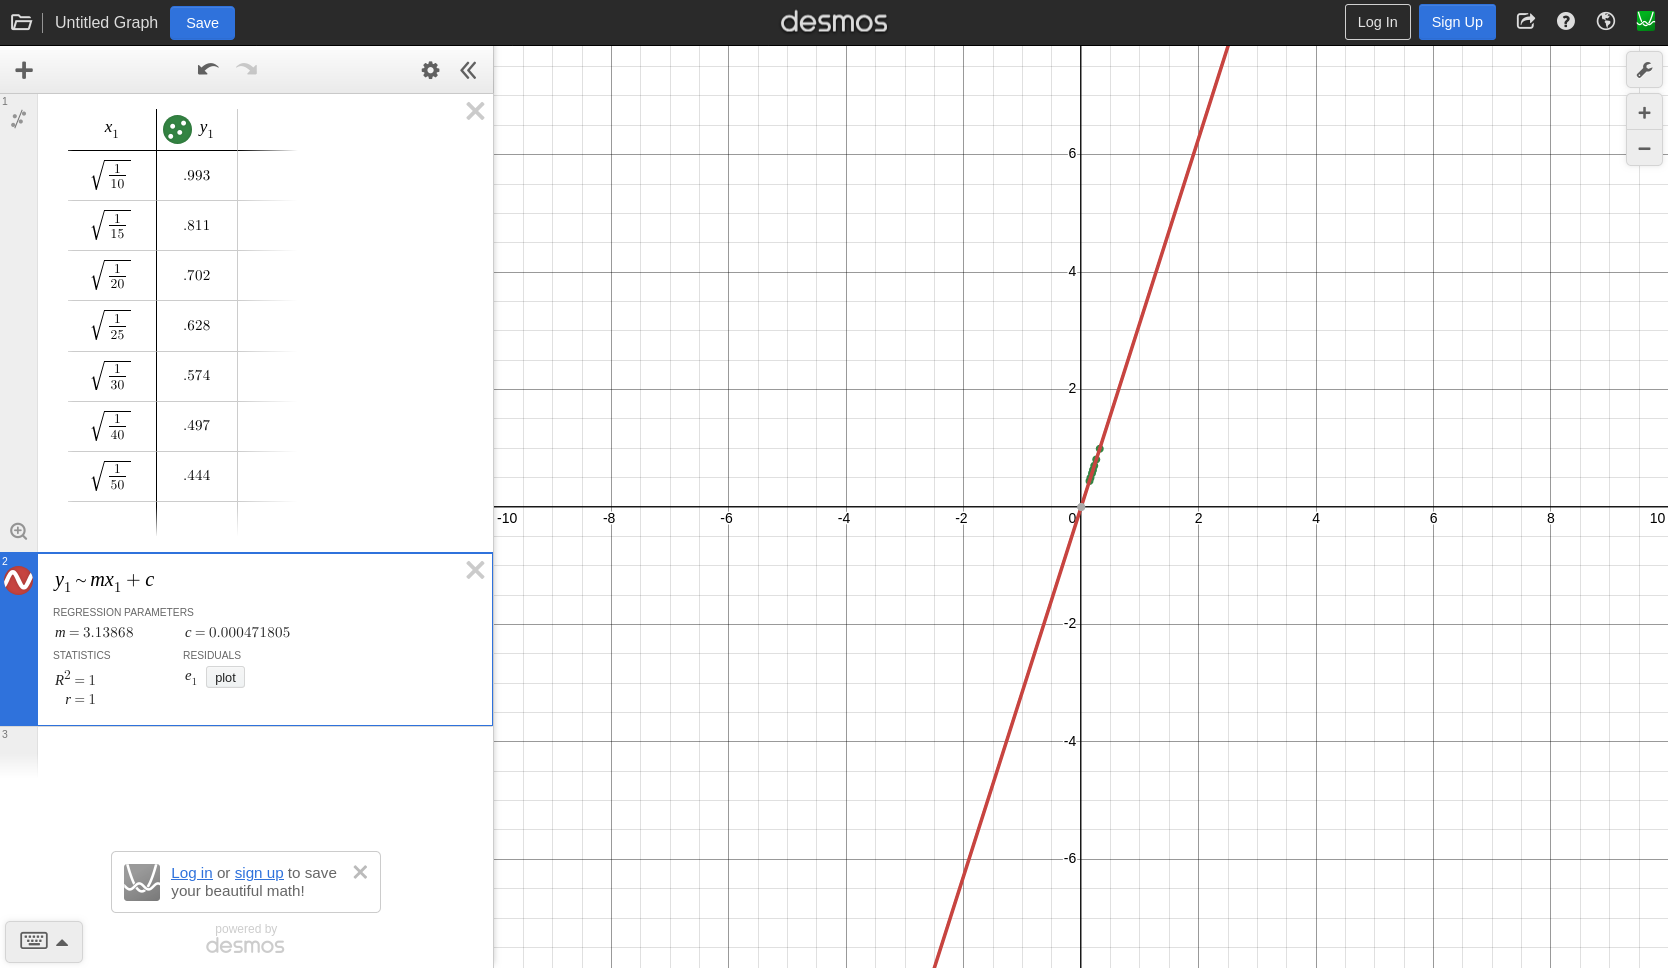
\includegraphics[width=\linewidth]{Screenshot 2025-09-05 at 21-05-25 Desmos Graphing Calculator.png}

	Part 2

	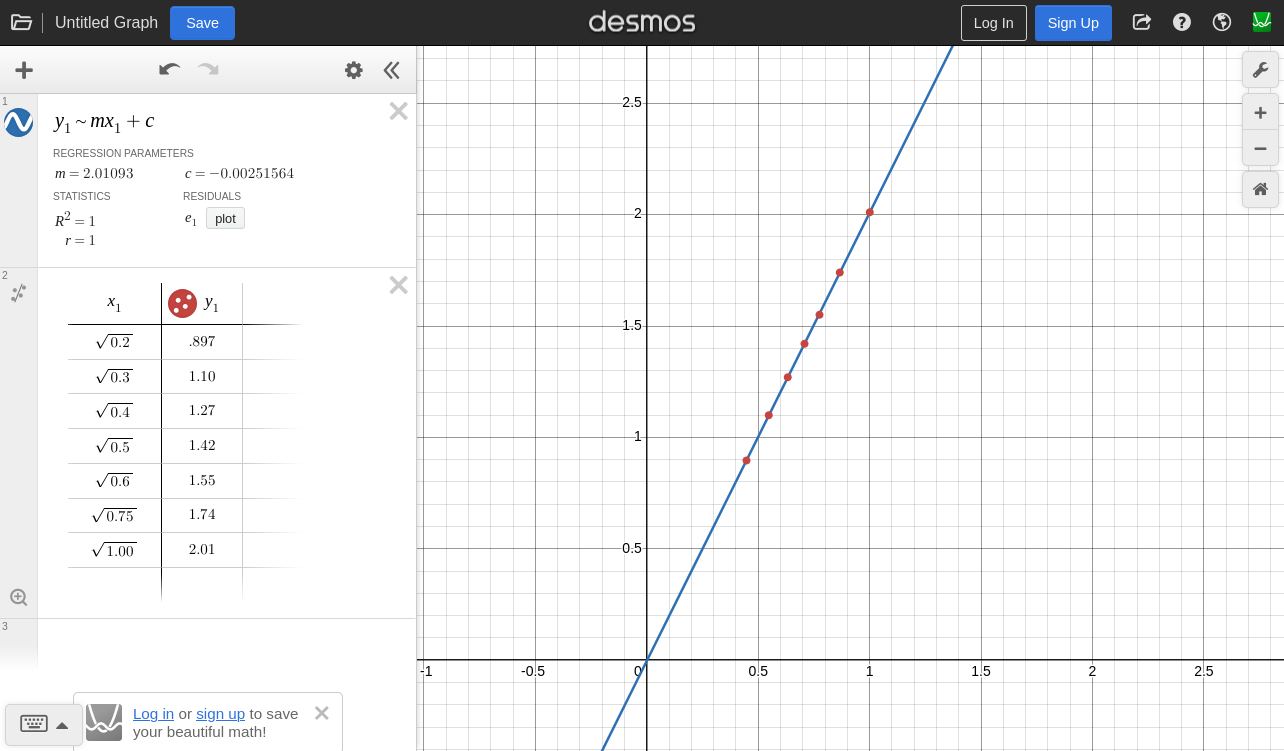
\includegraphics[width=\linewidth]{Screenshot 2025-09-05 at 09-21-45 Desmos Graphing Calculator.png}
\end{center}

\end{document}
